\section{Approach}

We have built and deployed a text-based social network where discussions form reply trees.\footnote{The platform and source code are publicly available; links are omitted for anonymous review.} Each post or reply passes through a three-stage LLM pipeline: \textbf{extraction}, \textbf{deduplication}, and \textbf{ranking}. Together these stages transform linear discussion threads into a structured argument graph that can be queried, navigated, and sorted by argument quality. Extraction uses Gemini 3.1 Flash Lite, deduplication uses Gemini 3 Flash, and embeddings use Gemini Embedding 001 (1536 dimensions).\footnote{Model identifiers: \texttt{gemini-3.1-flash-lite-preview}, \texttt{gemini-3-flash-preview}, \texttt{gemini-embedding-001}.}

\paragraph{Extraction.} An LLM decomposes each post or reply into individual argumentative discourse units (I-nodes) and identifies support and attack relations (S-nodes) between them, using few-shot prompting with no task-specific fine-tuning. Each I-node is rewritten in canonical form---resolving anaphora, expanding acronyms, and removing contextual dependencies---so that arguments can be compared across discussions.

\paragraph{Deduplication.} We adopt a retrieve-then-verify pattern---analogous to retrieval-augmented generation (RAG)---using an LLM as the verification step. Canonical I-node texts are embedded and, for each new I-node, we retrieve the $k$ nearest neighbours via HNSW search \citep{MalkovYashunin2016} and present them to an LLM for pairwise equivalence judgement. Confirmed matches are merged, linking the new text into the existing argument graph. Because HNSW supports incremental insertion, deduplication runs in $O(n \log n)$ as arguments arrive---unlike batch clustering approaches---and cross-thread merging transforms independent reply trees into an AIF-like hypergraph \citep{Chesnevar:2007:AIF} where the same claim can be supported or attacked from multiple discussions.

\paragraph{Ranking.} With arguments structured as a graph, the thread interface becomes a projection, and the key question becomes how to sort replies. We implement EvidenceRank, a PageRank \citep{pagerank:1999} variant for Quantitative Bipolar Argumentation Frameworks \citep{baroni-etal-2018-qbaf,albini-etal-2020-pagerank-argumentation}, where each I-node is seeded with its social vote score and iteratively updated through graph propagation: supporting neighbours increase a node's score while attacking neighbours decrease it. Reply-level scores are computed by summing constituent I-node scores, with a bridge multiplier rewarding replies that engage multiple distinct argument targets. Figure~\ref{fig:architecture} illustrates the full pipeline; complexity analysis is provided in Appendix~\ref{app:architecture}.

\begin{figure*}[t]
\centering
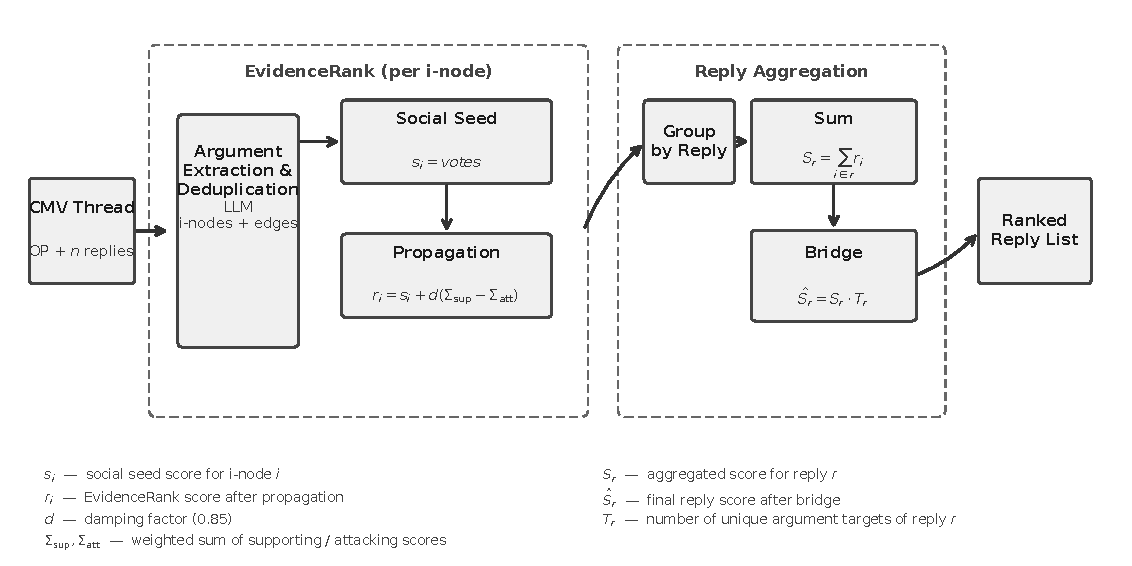
\includegraphics[width=\textwidth]{figures/architecture-er-vote-sum-nodc-bridge.pdf}
\caption{Architecture of the EvidenceRank pipeline showing argument extraction, graph propagation, and reply aggregation.}
\label{fig:architecture}
\end{figure*}
